\section{Electroosmotic flow}
As described in section \ref{sec:et:electroosmosis}, electroosmotic
flow is driven by an electric field rather than a pressure gradient.
Charge particles will be affected by a force and will drag the fluid
with them. The effect is investigated in this section.

A 10 $\mu$m channel is considered with walls charged with $3.56
\mu$C/m$^2$. The 1:1 ratio between positive and negative ions is in
this section put aside for a moment. To investigate how the
electroosmotic flow behaves for different situations of the charge
density, especially in the middle of the channel, the amount of
negative ions are varied. The different situations are investigated, a
surplus and a lack of negative ions together with a neutral solution
at the middle of the channel. Thus, the following values of the mean
concentration of negative ions are set: $0.7\C_0$, $0.75\C_0$,
$0.78\C_0$, $0.8\C_0$ and $0.85\C_0$. 

A constant electric field of $10^5$ V/m along the channel are set
and the same Peclet and Reynolds number as before are used. The
obtained ion concentrations and the velocity profiles are presented in
fig. \ref{fig:res:eo_charge} and fig. \ref{fig:res:eo_u}
respectively. 

\begin{figure}
\begin{center}
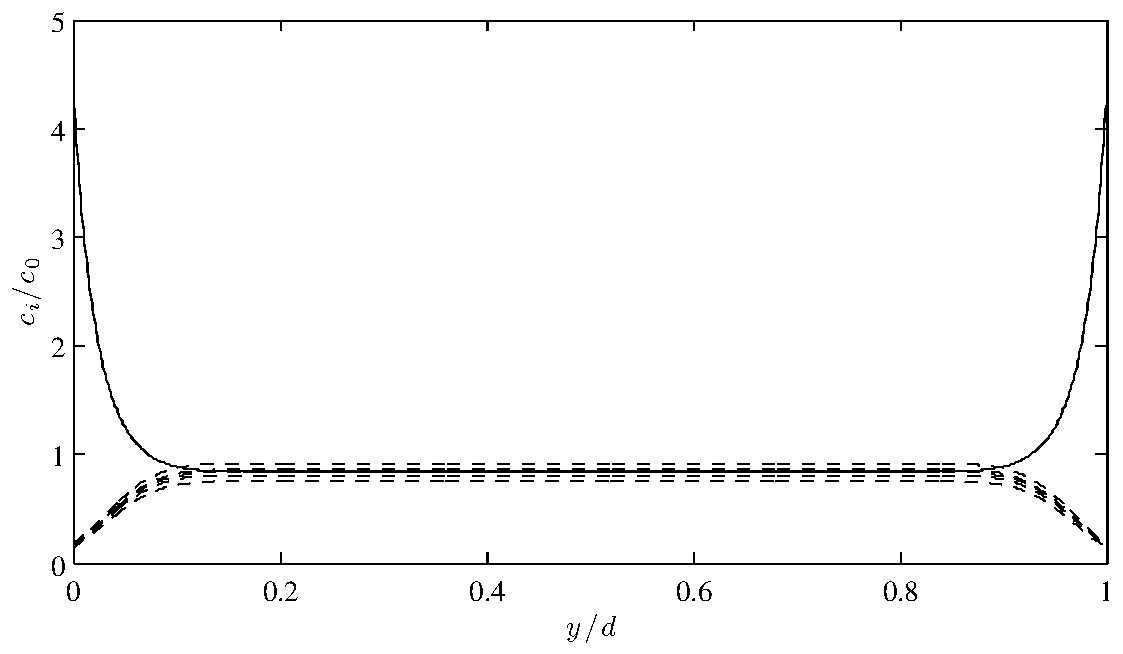
\includegraphics[width=0.9\textwidth]{fig/eo_conc.pdf}
\end{center}
\caption[Charge distributions for a varied ratio of positive and
  negative ions.]{Computed charge distributions for positive (solid)
  and negative (dashed) ions. The mean concentration of positive ions
  is $\C_0$ while that of negative ions are varied between the values
  $0.7\C_0$, $0.75\C_0$, $0.78\C_0$, $0.8\C_0$ and $0.85\C_0$. The
  geometry is a channel of width $10 \mu$m.}
\label{fig:res:eo_charge}
\end{figure}

\begin{figure}
\begin{center}
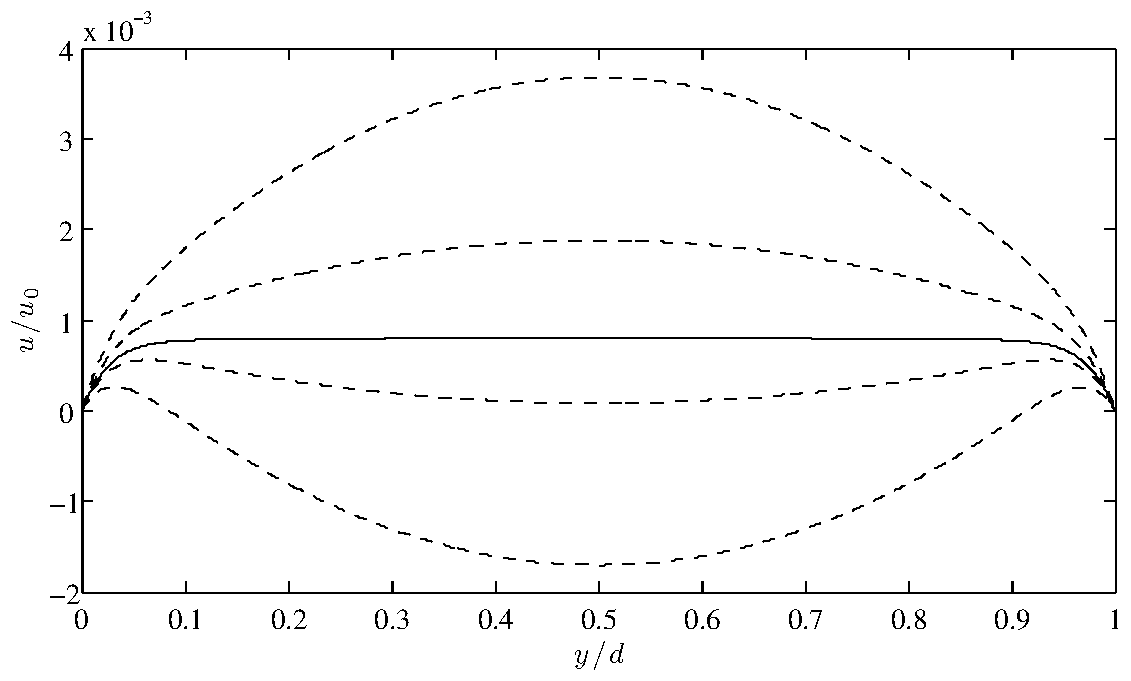
\includegraphics[width=0.9\textwidth]{fig/eo_u.pdf}
\end{center}
\caption[Computed velocity profiles for electroosmotic flow.]{Computed
  velocity profiles for electroosmotic flow, in a $10 \mu$m wide
  channel. The different profiles correspond to different ratios
  between positive and negative ions, see
  fig. \ref{fig:res:eo_charge}. The solid profile is the ``plug flow''
  that corresponds to the Poisson-Boltzmann case, where the middle of
  the channel is net neutrally charged.}
\label{fig:res:eo_u}
\end{figure}

In the case with a neutral middle of the channel the traditional
``plug profile'' of electroosmotic flow for wide channels are
reproduced. In this case the force from the electric field only
affects the fluid near the walls where a net charge is present, due to
viscous forces, a constant velocity profile is then obtained in the
middle of the channel. For a positive net charge in the middle of the
channel and thereby everywhere in the channel, the velocity profiles
are not of the ``plug'' shape but more parabolic. For a negatively net
charged middle of the channel and with the parameter of choice, the
viscous effect only compensates for the opposing effect from the
electric field when there is a small negative net charge. We see that
in this case, with the chosen parameters, for a 1:1 solution the flow
would be completely opposite of the electric field which is an
apparent difference to the wide channel case.
